
\documentclass{article} % For LaTeX2e
\usepackage{iclr2027_conference,times}

% Optional math commands from https://github.com/goodfeli/dlbook_notation.
\input{math_commands.tex}
\usepackage{url}
\usepackage{amsmath,amssymb,booktabs,microtype,multirow}
\usepackage{graphicx}
\usepackage{subcaption}
\captionsetup[table]{font={normalfont,normalsize},labelfont=normalfont,textfont=normalfont,justification=raggedright,singlelinecheck=false,position=above}
\usepackage[hidelinks]{hyperref}
\usepackage{float}
\usepackage{makecell}
\usepackage[table]{xcolor}

\definecolor{ThinkingBlue}{HTML}{EAF3FA}
\definecolor{GainGreen}{HTML}{18864B}
\definecolor{LossRed}{HTML}{C43D3D}

\title{From Perception to Integration: \\ Revisiting the Internal Dynamics of Reasoning in Vision-Language Models}

% Authors must not appear in the submitted version. They should be hidden
% as long as the \iclrfinalcopy macro remains commented out below.
% Non-anonymous submissions will be rejected without review.

\author{Antiquus S.~Hippocampus, Natalia Cerebro \& Amelie P. Amygdale \thanks{ Use footnote for providing further information
about author (webpage, alternative address)---\emph{not} for acknowledging
funding agencies.  Funding acknowledgements go at the end of the paper.} \\
Department of Computer Science\\
Cranberry-Lemon University\\
Pittsburgh, PA 15213, USA \\
\texttt{\{hippo,brain,jen\}@cs.cranberry-lemon.edu} \\
\And
Ji Q. Ren \& Yevgeny LeNet \\
Department of Computational Neuroscience \\
University of the Witwatersrand \\
Joburg, South Africa \\
\texttt{\{robot,net\}@wits.ac.za} \\
\AND
Coauthor \\
Affiliation \\
Address \\
\texttt{email}
}

% The \author macro works with any number of authors. There are two commands
% used to separate the names and addresses of multiple authors: \And and \AND.
%
% Using \And between authors leaves it to \LaTeX{} to determine where to break
% the lines. Using \AND forces a linebreak at that point. So, if \LaTeX{}
% puts 3 of 4 authors names on the first line, and the last on the second
% line, try using \AND instead of \And before the third author name.

\newcommand{\fix}{\marginpar{FIX}}
\newcommand{\new}{\marginpar{NEW}}
\newcommand{\Acc}{\operatorname{Acc}}

%\iclrfinalcopy % Uncomment for camera-ready version, but NOT for submission.
\begin{document}
\raggedbottom


\maketitle

\begin{abstract}
Vision-language models (VLMs) can recognize visual primitives, yet how explicit reasoning supports their joint use remains unclear. We investigate this question through cognitively inspired tasks that isolate individual visual judgments and combine them within a controlled Composite task. Across four models, behavioral evaluation, probing, and counterfactual state interventions show that primitive information is available without explicit reasoning and influences answer computation, while the composite answer becomes accessible as reasoning unfolds. Truncated-prefix evaluation further reveals that the accumulated reasoning can support a correct answer before natural termination. We train a lightweight hidden-state detector to predict answer readiness and use it to guide early stopping. Across MMStar and RealWorldQA, adaptive stopping reduces mean reasoning tokens by up to 86.9\% and improves accuracy by up to 15.2 percentage points. Our findings connect the internal development of visual reasoning to efficient answer generation.
\end{abstract}

\section{Introduction}

Human visual reasoning coordinates several perceptual functions to reach a decision. Recognizing an object, binding its features, estimating quantity, and understanding spatial relations each contribute information that may need to be combined. Cognitive science studies these functions through controlled tasks that isolate their demands \citep{treisman1980feature,feigenson2004core,logan1994spatial,kellman1991theory}. This approach offers a useful perspective on vision-language models (VLMs): understanding a complex visual answer requires examining both the component judgments and how the model uses them together.

Visual benchmarks assess perceptual and compositional abilities, while mechanistic studies locate visual information and trace its movement across model layers \citep{johnson2017clevr,huang2025visfactor,neo2025interpreting,zhang2025crossmodal}. A remaining question concerns the role of explicit reasoning between perception and answering. Success on individual judgments does not establish that a model can combine them, and success on the final answer does not reveal when the necessary combination occurred. We ask how a composite visual answer develops during native reasoning, and when the accumulated computation becomes sufficient to produce it.

To examine this process, we pair four tasks grounded in cognitive paradigms with a Composite task that brings their demands together. Feature Binding, Numerosity, Spatial Relations, and Amodal Completion isolate component judgments; comparing the numbers of red circles on two sides of an occluded scene requires their joint use. This design lets us examine what reasoning contributes once the component abilities have been established. Counterfactual pairs change the answer-determining property while controlling shared scene content \citep{gardner2020evaluating,bitton2021automatic}. They support matched comparisons of representations and interventions. Evaluating successive reasoning prefixes then reveals when the model can turn the accumulated information into a correct answer.

This analysis reveals a distinction between becoming ready to answer and choosing to finish reasoning. A prefix can already support accurate answering before the model naturally terminates, and generation beyond that prefix need not improve the answer. We refer to this prefix sufficiency as \emph{answer readiness}. The gap between readiness and termination exposes a form of overthinking and raises a practical question: can the model's evolving state identify when continued reasoning is no longer needed?

Answer readiness provides a target for this decision. Its measurement uses reference answers, but an inference-time stopping rule must operate without them. We therefore train a lightweight hidden-state detector to predict answer readiness and trigger answer generation, building on prior work on correctness- and sufficiency-based early exit \citep{zhang2025reasoningmodels,yang2026deer,xiang2026thinking}. Experiments on MMStar and RealWorldQA show that adaptive stopping substantially reduces reasoning length and can improve answer accuracy. Early stopping makes the study of visual answer formation actionable: the point at which reasoning supports an answer can also guide when to produce it.
\begin{figure}[H]
    \centering
    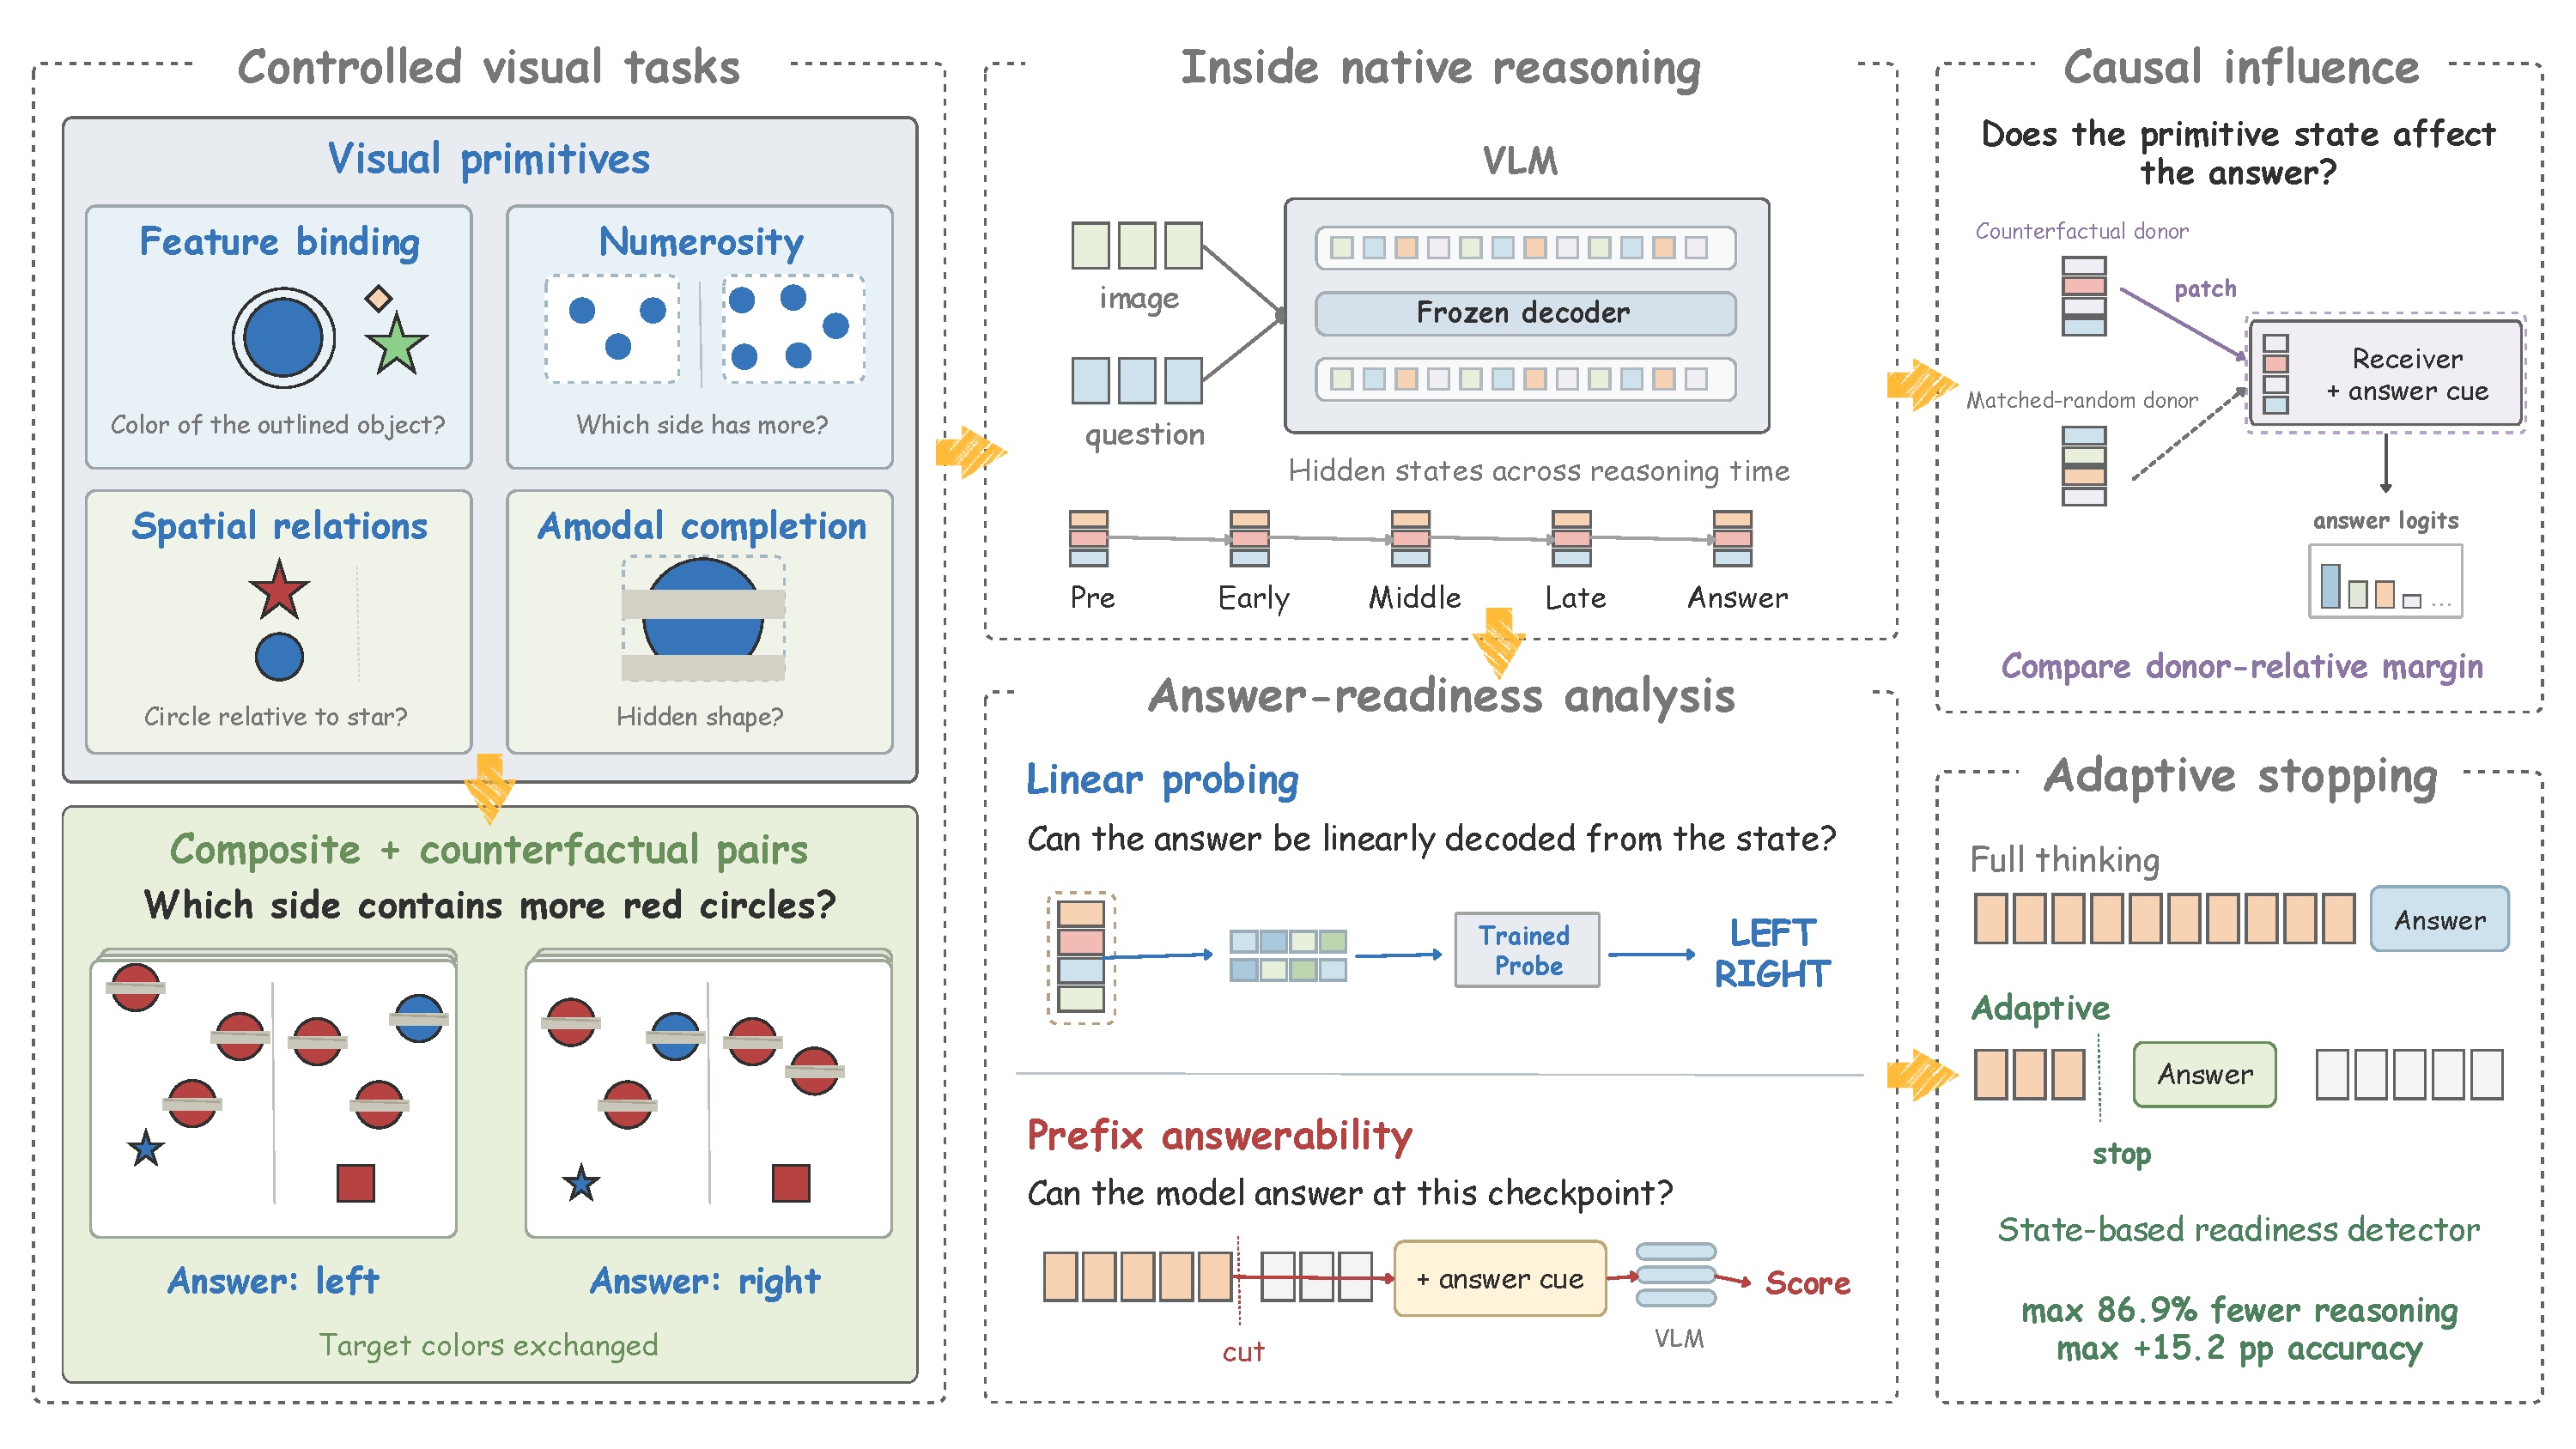
\includegraphics[width=1.02\linewidth]{figures/paper_overview.pdf}
    \caption{Overview of our study of answer formation in vision-language models. Left: Four controlled visual tasks and counterfactual Composite pairs separate primitive judgments from their joint use. Middle: Hidden-state probing and truncated-prefix evaluation track answer readiness during native reasoning. Right: Counterfactual state interventions test the causal influence of primitive visual representations, and a readiness detector enables adaptive early stopping.}
\end{figure}

\section{Related Work}

\paragraph{Multimodal reasoning and visual evaluation.}
Diagnostic benchmarks isolate compositional visual reasoning and cognitive abilities through controlled tasks \citep{johnson2017clevr,schiappa2024probing,huang2025visfactor}. Multimodal CoT methods instead develop reasoning procedures, including textual rationales and intermediate steps grounded in image regions or objects \citep{zhang2024multimodalcot,shao2024visualcot,li2025vocot}. MME-CoT evaluates the quality, robustness, and efficiency of these reasoning processes, showing that additional thinking can have different effects on perception and reasoning tasks \citep{jiang2025mmecot}. We use controlled primitive and Composite tasks to examine how component judgments become available for a joint decision during native reasoning.

\paragraph{Interpreting visual representations in VLMs.}
Causal tracing and token interventions locate visual information and examine its contribution to VLM predictions \citep{basu2024understanding,neo2025interpreting}. Information-flow studies analyze how image content reaches question and answer positions \citep{zhang2025crossmodal}; subsequent work identifies task-dependent direct and text-mediated pathways and distinguishes ordinary routing from fallback behavior under intervention \citep{salazar2026pathways}. Layer-wise probing further separates visual grounding, semantic processing, and answer formatting \citep{yu2025multimodal}. We use probing and state interventions to examine the availability and causal influence of primitive visual information without explicit reasoning. We then track Composite answer decodability and answer readiness across reasoning time.

\paragraph{Efficient reasoning and early exit.}
Hidden-state probes can predict eventual reasoning success \citep{afzal2025knowing} or verify intermediate answers and support early exit \citep{zhang2025reasoningmodels}. DEER uses trial-answer confidence to decide when to stop, while DTSR assesses the sufficiency of the accumulated reasoning \citep{yang2026deer,xiang2026thinking}. In VLMs, \citet{bi2026seeing} probe reasoning helpfulness and desired generation length, then control behavior through attention-head interventions. Our stopping target is whether the current prefix supports a correct answer under immediate forced answering. We learn this target from truncated traces and use a hidden-state detector to stop online, applying the answer-readiness finding from our controlled visual analysis.
\section{Interpreting Composite Visual Reasoning}
\label{sec:interpretability}

This section examines how component visual judgments support the formation of a composite answer. We introduce the controlled tasks and counterfactual pairs, examine the behavioral performance, decodability, and causal role of the component judgments, and then trace how the Composite answer develops during reasoning.

\subsection{Interpretability Analysis Setup}
\label{sec:primitive}

\paragraph{Feature Binding.}
Feature Binding associates visual attributes with the objects that carry them. Human illusory-conjunction errors show that individual features can be perceived yet incorrectly combined across objects, motivating the distinction between detecting an attribute and binding it to its source \citep{treisman1980feature,treisman1982illusory}. Each image contains multiple colored shapes, with one object marked by a black outline; the model identifies its color. The task measures whether the model associates the queried attribute with the designated object.

\paragraph{Numerosity.}
Numerosity concerns the quantities of non-symbolic sets \citep{feigenson2004core}. Infant studies demonstrate quantity discrimination before symbolic counting, with controls for continuous visual properties needed to distinguish numerical sensitivity from responses to physical extent \citep{xu2000large}. The model compares dot arrays on opposite sides of a divider and selects the side containing more dots. We control the relationship between numerosity and total dot area, while the left/right answer format avoids requiring an exact numerical response.

\paragraph{Spatial Relations.}
Spatial Relations specify the position of a target relative to a reference object \citep{carlson1999what}. Human spatial-relation judgments depend on attentional selection, motivating explicit designation of the objects whose relation is queried \citep{logan1994spatial}. Black and gray outlines designate these two roles, respectively, while object colors and shapes vary across images. The model identifies whether the target is left, right, above, or below the reference, requiring it to distinguish the marked roles and judge their relative positions.

\paragraph{Amodal Completion.}
Amodal Completion concerns perceiving a whole object from the visible portions of an occluded shape \citep{kellman1991theory}. Priming studies show that a partly occluded object can activate its completed interpretation, supporting a distinction between representing visible fragments and the whole shape \citep{sekuler1992perception}. We partially occlude a geometric shape and ask the model to identify the complete shape from candidate answers. This task assesses shape recognition under occlusion, providing the component judgment needed to identify partially hidden objects in the Composite task.

\paragraph{Composite Task.}
The Composite task asks which side of a divider contains more red circles among colored and partially occluded shapes. It combines shape recognition under occlusion, color--shape binding, left/right region assignment, and comparison of the resulting target counts. This task allows us to examine how component judgments support a single decision during reasoning.


\paragraph{Counterfactual Pairs.}
For mechanistic comparisons, matched counterfactual pairs vary an answer-determining visual property while preserving the corresponding scene context \citep{gardner2020evaluating,bitton2021automatic}. Feature Binding, Numerosity, and Spatial Relations use separate single-image and intervention-pair datasets; Amodal Completion and Composite are constructed as paired datasets. These pairs provide matched contrasts for analysis and donor--receiver examples for state interventions. Dataset construction, control conditions, and splits are provided in Appendix~\ref{app:data_generation}.

\begin{figure}[H]
    \centering
    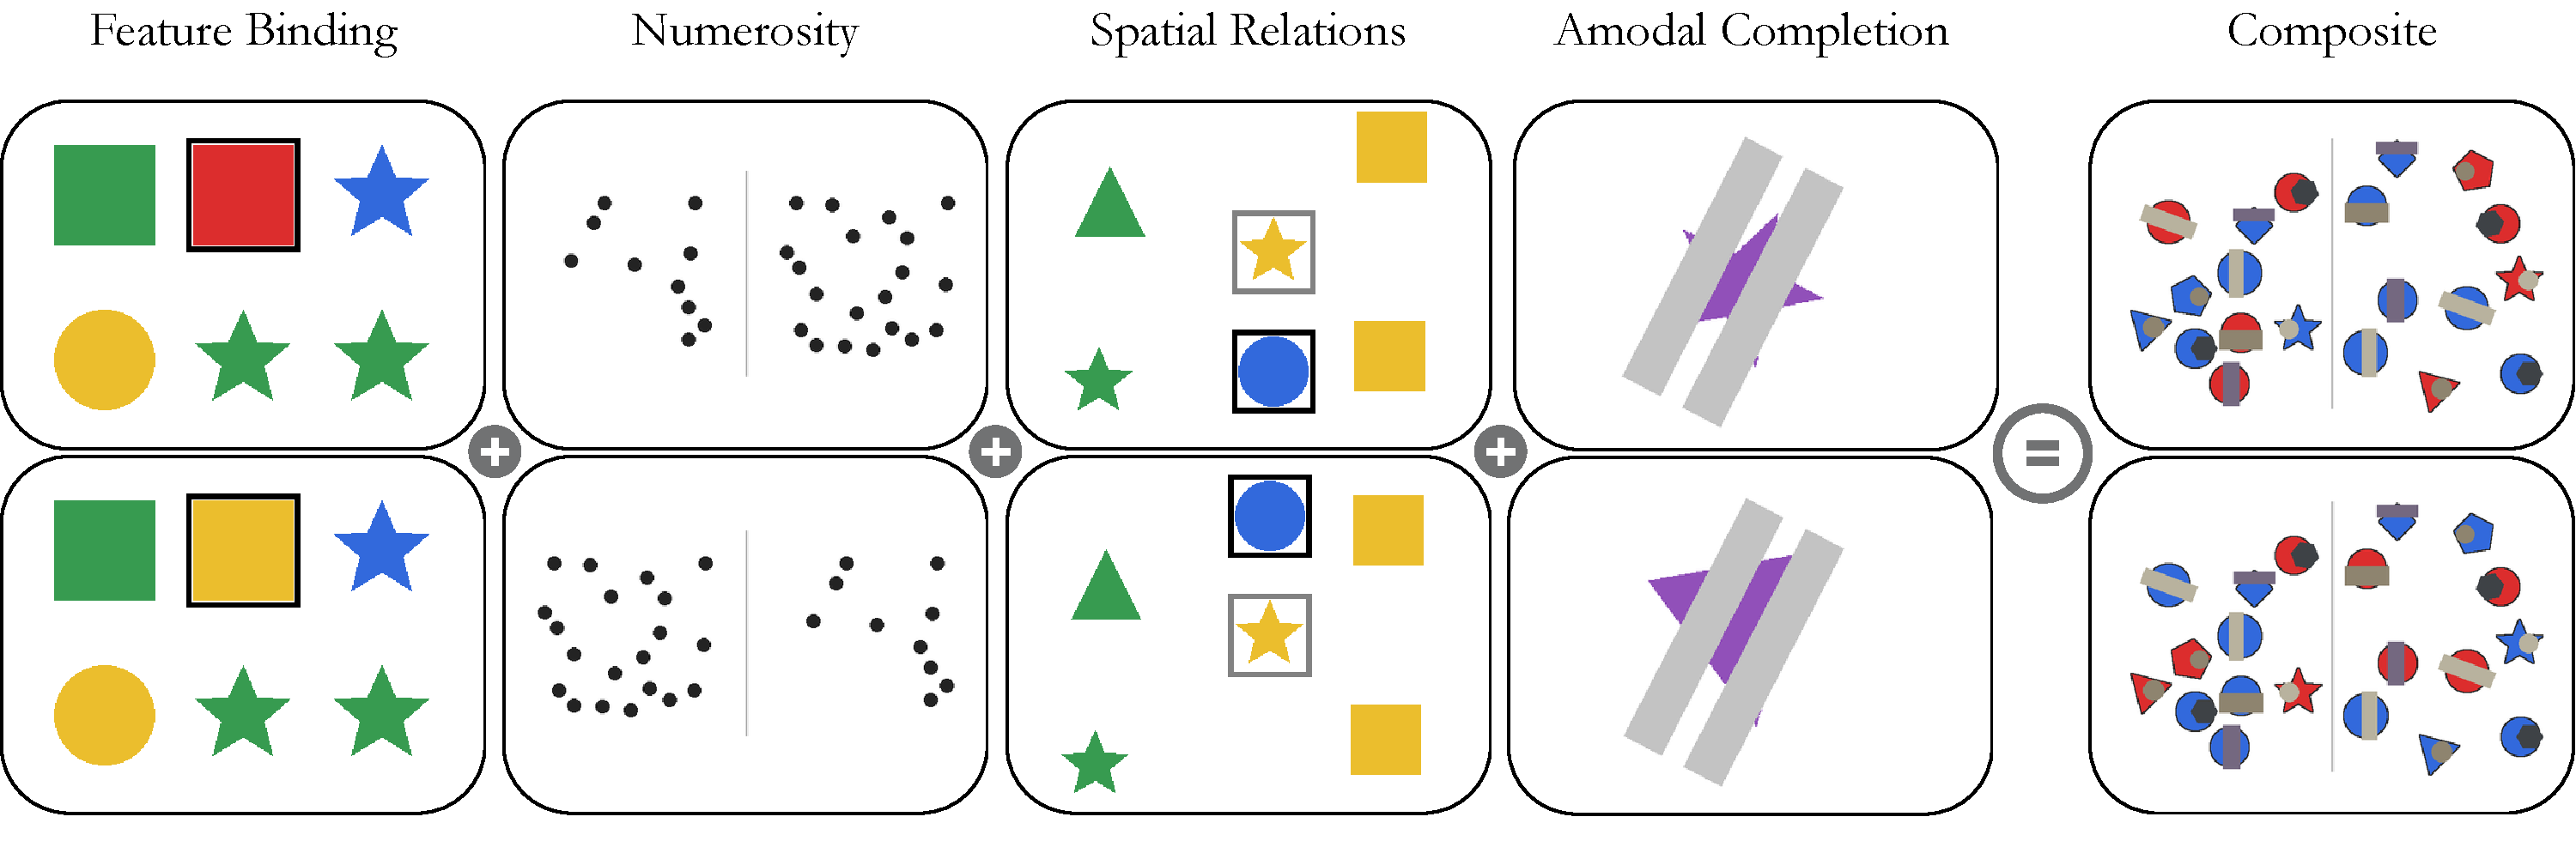
\includegraphics[width=\textwidth]{figures/Controlled visual tasks.pdf}
    \caption{\textbf{Controlled visual tasks.} Each column shows a counterfactual pair in which the task-relevant visual variable and correct answer change together.}
    \label{fig:dataset_examples}
\end{figure}


\subsection{Visual Primitives Are Already Available Without Reasoning}
\label{sec:answer_ready_states}

We first ask whether models possess the component visual abilities needed for the Composite task without generating explicit reasoning. Behavioral evaluation tests whether they can perform the individual judgments; layer-wise linear readouts test whether the corresponding variables are recoverable from internal representations; counterfactual state interventions test how those representations affect answering \citep{belinkov2021probing}.

\paragraph{Behavioral competence.}
We keep model parameters frozen, disable thinking, and ask each model to answer the four primitive tasks directly. Table~\ref{tab:primitive_behavior} shows that all four models exceed the task-specific chance levels. Performance is higher on Feature Binding and Spatial Relations, while Numerosity and Amodal Completion produce more errors. These results establish that the models can perform the component judgments without an explicit reasoning trace.

\begin{table}[H]
    \centering
    \small
    \setlength{\tabcolsep}{4.5pt}
    \caption{\textbf{All four component judgments can be performed above chance without explicit reasoning.} Answer accuracy (\%) is evaluated on 1,000 images per task and model. Chance is uniform guessing over the answer choices: two for Numerosity and four for the other tasks.}
    \label{tab:primitive_behavior}
    \begin{tabular}{lccccc}
        \toprule
        Task
        & Qwen3.5 4B
        & Qwen3.5 9B
        & Gemma 4 4B
        & Gemma 4 12B
        & Chance \\
        \midrule
        Feature Binding
        & 98.0
        & 99.8
        & 98.6
        & 99.9
        & 25.0 \\
        Numerosity
        & 79.6
        & 85.2
        & 72.4
        & 86.5
        & 50.0 \\
        Spatial Relations
        & 99.8
        & 100.0
        & 97.5
        & 89.5
        & 25.0 \\
        Amodal Completion
        & 76.8
        & 80.5
        & 81.4
        & 72.9
        & 25.0 \\
        \bottomrule
    \end{tabular}
\end{table}



\paragraph{Layer-wise decodability.}
To locate the relevant visual information, we mean-pool image-token hidden states at each layer:
\begin{equation}
    v_i^{(\ell)}=\frac{1}{|\mathcal I_i|}
    \sum_{t\in\mathcal I_i}h_{i,t}^{(\ell)},
\end{equation}
where $h_{i,t}^{(\ell)}$ is the representation of sample $i$ at layer $\ell$ and token position $t$, and $\mathcal I_i$ contains its image-token positions. We standardize these vectors using training-set statistics to obtain $z_i^{(\ell)}$, whose rows form the training matrix $Z_\ell$. For each model and task, we fit an independent ridge linear readout at every layer, keeping the VLM frozen and fitting only the readout matrix:
\begin{equation}
    W_\ell^*=\arg\min_W\|Z_\ell W-Y\|_F^2+\lambda\|W\|_F^2,
    \qquad
    \hat y_i=\arg\max_c\bigl(z_i^{(\ell)}W_\ell^*\bigr)_c.
\end{equation}
Here $Y$ contains one-hot semantic labels: target color, the more numerous side, spatial direction, or complete shape, depending on the task; $\lambda$ controls regularization.

We evaluate each readout on held-out samples, keeping both members of a pair in the same split for paired data. To distinguish visual information from cues in the question, we independently fit the same readout on mean-pooled question-token states from inputs without an image. The four semantic label spaces contain four, two, four, and six classes, respectively. In particular, the Amodal Completion readout predicts one of six complete shapes, whereas behavioral evaluation selects among the four candidates presented in each question. Split sizes and fitting details appear in Appendix~\ref{app:primitive_analysis}.

\begin{figure}[H]
    \centering
    
\includegraphics[width=0.96\textwidth]{figures/primitive_decodability_legend.png}
    \par\vspace{-2pt}

    \begin{subfigure}[t]{0.238\textwidth}
        \centering
        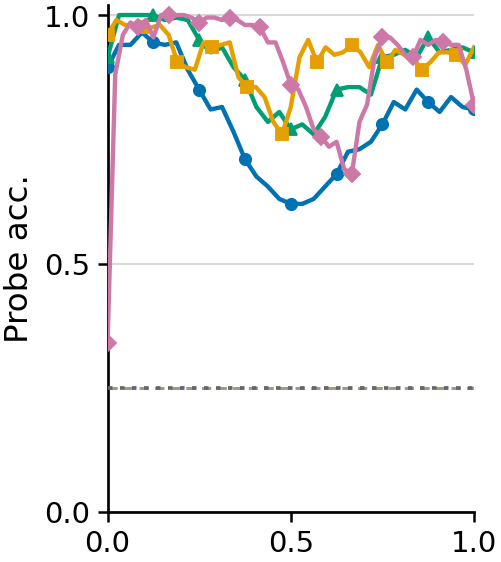
\includegraphics[width=\linewidth]{figures/primitive_decodability_feature_binding.png}
        \caption{Feature Binding}
    \end{subfigure}\hfill
    \begin{subfigure}[t]{0.238\textwidth}
        \centering
        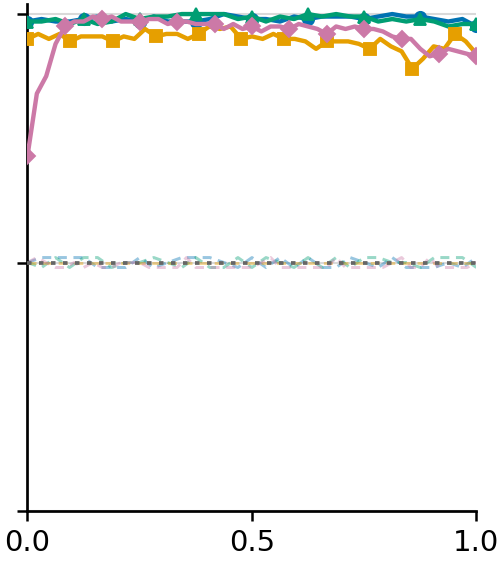
\includegraphics[width=\linewidth]{figures/primitive_decodability_numerosity.png}
        \caption{Numerosity}
    \end{subfigure}\hfill
    \begin{subfigure}[t]{0.238\textwidth}
        \centering
        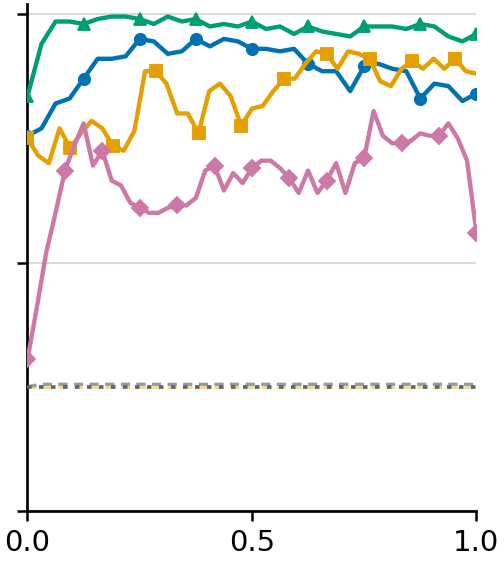
\includegraphics[width=\linewidth]{figures/primitive_decodability_spatial_relations.png}
        \caption{Spatial Relations}
    \end{subfigure}\hfill
    \begin{subfigure}[t]{0.238\textwidth}
        \centering
        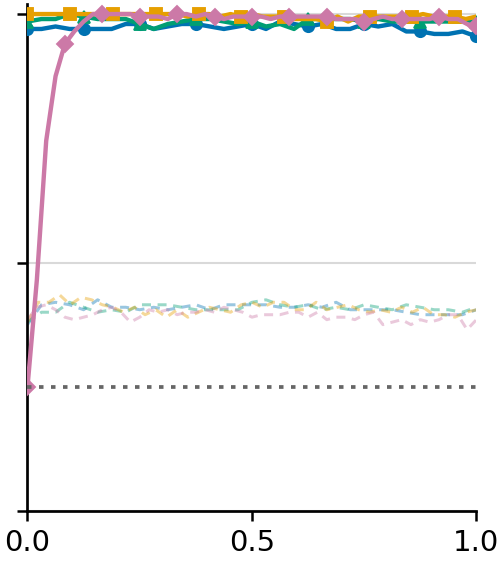
\includegraphics[width=\linewidth]{figures/primitive_decodability_amodal_completion.png}
        \caption{Amodal Completion}
    \end{subfigure}

    \caption{Controlled visual variables are decodable across model depth.
    Solid curves show held-out accuracy from image-conditioned probes; dashed
    curves show question-only controls. Gray dotted lines mark task-specific
    chance accuracy. Normalized layer depth is the layer index divided by the
    largest tested layer index for each model.}
    \label{fig:primitive_decodability}
\end{figure}

Figure~\ref{fig:primitive_decodability} shows that the visual variables are linearly recoverable across multiple depths, with task- and model-dependent profiles. Numerosity and complete-shape readouts achieve high accuracy, while Feature Binding and Spatial Relations vary more with depth. Question-only controls are approximately at chance for the first three tasks. For Amodal Completion, the varying candidate list provides partial information about the shape label, raising the control above chance. Image-conditioned readouts exceed this control through most layers, indicating recoverable visual information in the states. We next test how replacing these states affects answering.

\paragraph{Causal influence.}
For each counterfactual pair, we treat one sample as the receiver and the other, whose correct answer differs, as the donor. At the input to a selected decoder block, we replace the receiver's image-token states with the corresponding donor states and resume the forward pass:
\begin{equation}
    H_{r,\mathcal I_r}^{(\ell)}\leftarrow H_{d,\mathcal I_d}^{(\ell)}.
\end{equation}
We intervene in both directions and retain pairs for which both original answers are correct under the intervention scoring protocol. A matched-random donor comes from another pair with the receiver's semantic label and supplies states at the same token region. Model parameters remain frozen throughout; patching requires no additional training.

Logit differences capture partial effects of activation patching even when the predicted answer does not change \citep{heimersheim2024activation}. We use the donor-relative margin $m=s(y_d)-s(y_r)$, where $s(y)$ is the candidate answer logit score and $y_d$ and $y_r$ are the donor and receiver answers. To summarize how consistently interventions move the scores toward the donor, we report the difference between the proportions of targeted and matched-random replacements that increase this margin over the unpatched receiver:
\begin{equation}
    \Delta_{\mathrm{patch}}=100\left[
    \Pr(m_{\mathrm{target}}>m_{\mathrm{base}})
    -\Pr(m_{\mathrm{random}}>m_{\mathrm{base}})
    \right].
\end{equation}
Here $m_{\mathrm{base}}$ is the unpatched receiver margin. Positive $\Delta_{\mathrm{patch}}$ indicates that counterfactual replacement increases the donor-relative margin more often than the control. This percentage-point difference measures the frequency of directional effects, rather than their magnitude or the rate of answer flips. Answer scoring and matching criteria appear in Appendix~\ref{app:primitive_analysis}.

\begin{figure}[H]
    \centering
    
\includegraphics[width=0.72\textwidth]{figures/primitive_causal_legend.png}
    \par\vspace{-2pt}

    \begin{subfigure}[t]{0.238\textwidth}
        \centering
        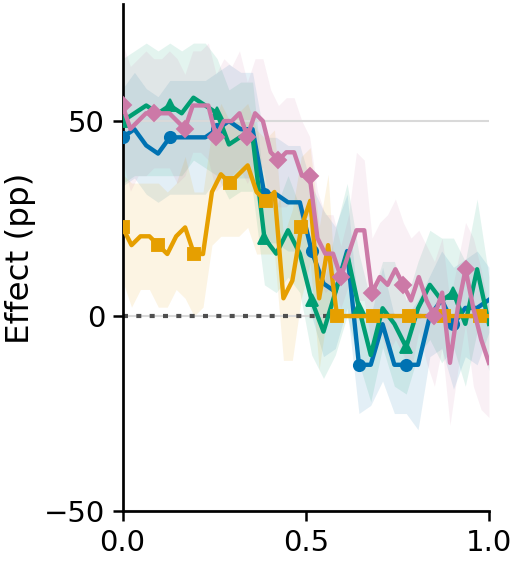
\includegraphics[width=\linewidth]{figures/primitive_causal_feature_binding.png}
        \caption{Feature Binding}
    \end{subfigure}\hfill
    \begin{subfigure}[t]{0.238\textwidth}
        \centering
        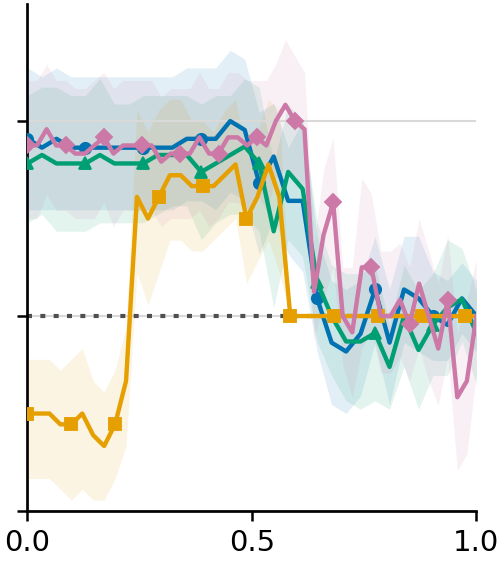
\includegraphics[width=\linewidth]{figures/primitive_causal_numerosity.png}
        \caption{Numerosity}
    \end{subfigure}\hfill
    \begin{subfigure}[t]{0.238\textwidth}
        \centering
        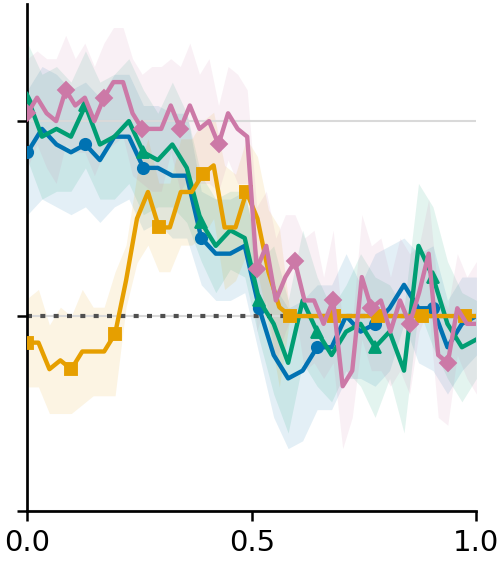
\includegraphics[width=\linewidth]{figures/primitive_causal_spatial_relations.png}
        \caption{Spatial Relations}
    \end{subfigure}\hfill
    \begin{subfigure}[t]{0.238\textwidth}
        \centering
        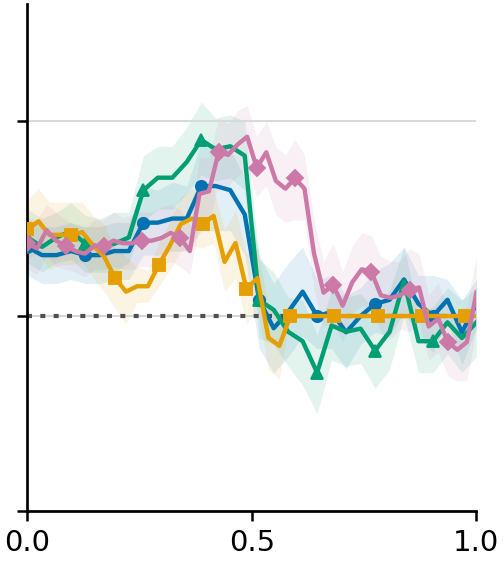
\includegraphics[width=\linewidth]{figures/primitive_causal_amodal_completion.png}
        \caption{Amodal Completion}
    \end{subfigure}

    \caption{Controlled visual variables exert depth-localized causal effects.
    Each curve reports the percentage-point difference between task-targeted
    and matched-random moves-toward-donor rates in the image-token region.
    Shaded bands are paired-bootstrap 95\% confidence intervals over matched
    pairs. Normalized layer depth is defined as in
    Figure~\ref{fig:primitive_decodability}.}
    \label{fig:primitive_causal}
\end{figure}

Figure~\ref{fig:primitive_causal} shows that targeted patching shifts scores toward the donor more consistently relative to the control in early-to-middle layers than at the final tested block. Visual variables remain decodable across depth, while patching effects are more localized. Together, these results establish component competence and answer-relevant visual states without explicit reasoning.

\subsection{Composite Answer Readiness Develops During Reasoning}

We now examine how native thinking supports a Composite decision and when the accumulated reasoning becomes sufficient to answer.

\paragraph{Reasoning improves counterfactual consistency.}
We compare no-thinking and native-thinking responses on the same held-out pairs. Sample accuracy scores individual images; pair-consistent accuracy requires both counterfactual members to be correct.

\begin{table}[H]
    \centering
    \small
    \renewcommand{\arraystretch}{1.15}
    \setlength{\tabcolsep}{2pt}
    \caption{\textbf{Native thinking improves counterfactual consistency.}
    Main values report accuracy (\%); brackets show pair-bootstrap 95\% confidence intervals.
    $\Delta$ is the change from answering without reasoning to answering with reasoning in percentage points. Budget hit reports the number and percentage of the 200 thinking-mode runs that reach the generation limit.}
    \label{tab:thinking_behavior}

    \begin{tabular*}{\textwidth}{
        @{\extracolsep{\fill}}
        l
        ccc
        ccc
        c@{}
    }
        \toprule
        & \multicolumn{3}{c}{\textbf{Sample Accuracy}}
        & \multicolumn{3}{c}{\textbf{Pair-Consistent Accuracy}} & \textbf{Budget hit} \\
        \cmidrule(lr){2-4}
        \cmidrule(lr){5-7}\cmidrule(lr){8-8}
        Model
        & Non-thinking
        & \textbf{Thinking}
        & $\Delta$
        & Non-thinking
        & \textbf{Thinking}
        & $\Delta$ & Count (\%) \\
        \midrule

        Qwen3.5 4B
        & \makecell{58.5\\{\scriptsize [53.0,64.0]}}
        & 
          \makecell{\textbf{80.0}\\{\scriptsize [74.0,86.0]}}
        & \textcolor{GainGreen}{$\uparrow\,21.5$}
        & \makecell{26.0\\{\scriptsize [18.0,35.0]}}
        & 
          \makecell{\textbf{67.0}\\{\scriptsize [58.0,76.0]}}
        & \textcolor{GainGreen}{$\uparrow\,41.0$} & 38 (19.0\%) \\

        Qwen3.5 9B
        & \makecell{66.5\\{\scriptsize [61.5,71.5]}}
        & 
          \makecell{\textbf{94.0}\\{\scriptsize [90.5,97.0]}}
        & \textcolor{GainGreen}{$\uparrow\,27.5$}
        & \makecell{36.0\\{\scriptsize [27.0,45.0]}}
        & 
          \makecell{\textbf{89.0}\\{\scriptsize [83.0,95.0]}}
        & \textcolor{GainGreen}{$\uparrow\,53.0$} & 11 (5.5\%) \\

        Gemma 4 4B
        & \makecell{52.0\\{\scriptsize [49.0,55.0]}}
        & 
          \makecell{\textbf{73.5}\\{\scriptsize [67.0,80.0]}}
        & \textcolor{GainGreen}{$\uparrow\,21.5$}
        & \makecell{7.0\\{\scriptsize [2.0,12.0]}}
        & 
          \makecell{\textbf{57.0}\\{\scriptsize [47.0,67.0]}}
        & \textcolor{GainGreen}{$\uparrow\,50.0$} & 0 (0.0\%) \\

        Gemma 4 12B
        & \makecell{\textbf{57.5}\\{\scriptsize [54.0,61.0]}}
        & 
          \makecell{54.5\\{\scriptsize [47.0,62.0]}}
        & \textcolor{LossRed}{$\downarrow\,3.0$}
        & \makecell{15.0\\{\scriptsize [8.0,22.0]}}
        & 
          \makecell{\textbf{34.0}\\{\scriptsize [25.0,43.0]}}
        & \textcolor{GainGreen}{$\uparrow\,19.0$} & 84 (42.0\%) \\

        \bottomrule
    \end{tabular*}
\end{table}

Table~\ref{tab:thinking_behavior} shows that native thinking improves pair-consistent accuracy across all four models. Sample accuracy also improves for three models, while Gemma 4 12B declines despite its higher pair consistency. This model also frequently reaches the generation limit, although the comparison does not isolate budget exhaustion as the cause of its lower sample accuracy. These final-response results leave open a temporal question: does the model accumulate enough information to answer before it finishes its full reasoning trace?

\paragraph{Tracing answer formation through thinking.}
We follow native traces at five checkpoints: before reasoning (\textsc{Pre}), at its early and middle stages, at the last reasoning token (\textsc{Late}), and immediately before the final choice token (\textsc{Answer}). For each model, validation pairs select a layer using pre-reasoning answer decodability; we then hold that layer fixed across checkpoints and test samples. Trajectory analysis retains pairs whose two traces provide usable checkpoints and a parsed answer, so its sample counts can differ from the full behavioral evaluation. Exact positions, selected layers, and split construction appear in Appendix~\ref{app:reasoning_checkpoints} and Appendix~\ref{app:data_generation}.

At each checkpoint, we fit an independent ridge linear readout to the hidden state at the selected layer and token position. The target is the correct Composite answer, left or right. The VLM remains frozen, and only the readout is fitted using the standardized features and ridge objective defined in Section~\ref{sec:answer_ready_states}. Each checkpoint's readout is trained and tested on the corresponding states from the same pair-preserving splits. Its held-out accuracy measures whether the correct answer can be recovered from that state.

To measure whether the accumulated prefix supports answering, we truncate each trace at the checkpoint, append a fixed answer suffix, and score the two candidate answers with the frozen model:
\begin{equation}
    \hat y_{i,t}^{\mathrm{suffix}}
    =\arg\max_{c\in\{\mathrm{left},\mathrm{right}\}}
    s_\theta(c\mid x_i,r_{i,\leq t},a),
    \qquad
    U(t)=\frac{1}{N}\sum_{i=1}^{N}
    \mathbf{1}[\hat y_{i,t}^{\mathrm{suffix}}=y_i].
\end{equation}
Here $x_i$ is the original image and prompt, $r_{i,\leq t}$ is the generated prefix through checkpoint $t$, $a$ is the fixed answer suffix, and $s_\theta$ is the candidate logit score. The suffix specifies the answer format without supplying the answer. We operationalize answer readiness through this prefix-conditioned accuracy: the probe reads a single hidden state, whereas $U(t)$ evaluates answering from the complete retained prefix, including any verbalized intermediate results.

\begin{figure}[H]
    \centering
    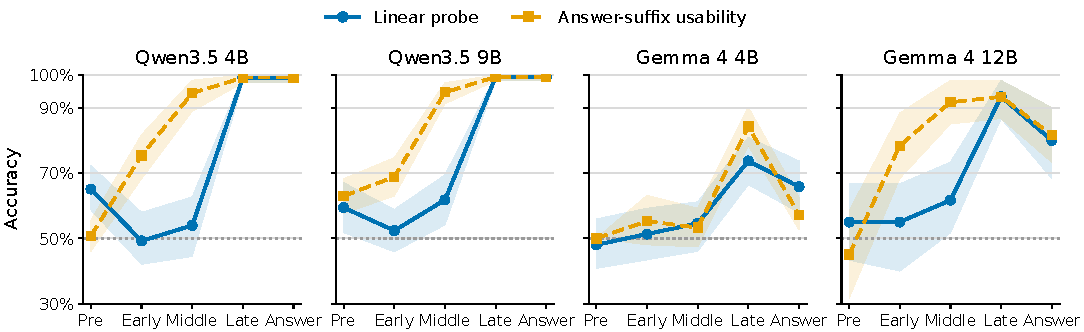
\includegraphics[width=\textwidth]{figures/answer_state_dynamics.pdf}
    \caption{\textbf{Answer readiness develops over native thinking.} Each panel follows one model through five reasoning checkpoints. Blue curves report held-out linear-probe accuracy for the final Composite answer from a fixed-depth hidden state. Orange curves report answer accuracy after truncating the native reasoning trace at the corresponding checkpoint and appending a fixed answer suffix. Shaded regions show pair-bootstrap 95\% confidence intervals; the horizontal dotted line marks binary chance.}
    \label{fig:answer_state_dynamics}
\end{figure}

\paragraph{Answer readiness develops during native thinking.}
Figure~\ref{fig:answer_state_dynamics} shows that answer decodability and prefix-conditioned answering are not consistently high across models before reasoning. Both improve as reasoning proceeds, but at different rates: prefix-conditioned accuracy rises earlier for the Qwen models and Gemma 4 12B, while Gemma 4 4B improves later. By \textsc{Late}, both measurements are high across all four models. Thus, the Composite answer becomes more recoverable from hidden states and more accessible through prefix-conditioned answering during native reasoning.

Moving from the last reasoning token (\textsc{Late}) to the position before the final choice (\textsc{Answer}) does not uniformly improve either measurement. Both Qwen models retain high performance, while both Gemma models decline at the final checkpoint. A prefix at the end of reasoning can therefore already support accurate answering, with no consistent improvement during the transition to the final response. This raises the practical question addressed next: can the evolving hidden state identify when to transition from reasoning to answering?

\section{Answer-Readiness-Guided Early Stopping}
\label{sec:early_stopping}

We turn prefix answer readiness into an online stopping decision using a lightweight detector, trained separately for each model and dataset at the layers selected on Composite.

\paragraph{Learning answer readiness.}
We truncate native traces at regular checkpoints, insert a fixed final-answer transition, and label each checkpoint by whether the frozen model's resulting answer is correct. The detector reads the current state, its change since the preceding checkpoint, and elapsed reasoning length:
\begin{equation}
    x_t=[h_t^{(\ell)};\ d_t^{(\ell)};\ t/B],
    \qquad p_t=\sigma(w^\top\tilde x_t+b),
\end{equation}
where $d_t^{(\ell)}$ is the change from the preceding checkpoint state, using a zero reference at the first checkpoint. $\tilde x_t$ uses training-set standardization, and $B$ is the generation budget. We freeze the VLM and fit only $w$ and $b$ with class-weighted binary cross-entropy. The target is correctness under immediate answering, not the outcome of the original full trace.

\paragraph{Online stopping.}
Every $\Delta=256$ reasoning tokens, the detector checks whether $p_t\geq\eta$ and triggers the same final-answer transition at the first crossing. Validation selects $\eta$ to minimize reasoning length within an accuracy-loss tolerance relative to full thinking. Without a crossing, generation continues to natural termination or the budget limit.

\paragraph{Evaluation.}
We evaluate 1,500 MMStar questions \citep{chen2024we} and 765 RealWorldQA questions \citep{xai2024realworldqa} using two-fold cross-validation, training and validating on one fold and testing on the other. Checkpoints from each question and duplicate RealWorldQA images stay together. Each question contributes one held-out prediction per condition. Full thinking and adaptive stopping share a $B=6{,}144$-token total budget; we compare final-answer accuracy and mean reasoning tokens under our common evaluation protocol. Training, splits, and scoring are detailed in Appendix~\ref{app:early_stopping}.

\subsection{Main Results}

\paragraph{MMStar.}
Adaptive stopping reduces reasoning length and improves accuracy for every model (Table~\ref{tab:early_stopping_main}), with the largest accuracy gain on Gemma 4 12B. Total output length also decreases across models, so savings extend beyond the reasoning segment. Total lengths and per-fold results appear in Appendix~\ref{app:stopping_results}.

\begin{table}[H]
    \centering
    \small
    \renewcommand{\arraystretch}{1.15}
    \setlength{\tabcolsep}{2pt}
    \caption{\textbf{Adaptive stopping reduces reasoning cost while improving MMStar accuracy.}
    Results are evaluated on all 1,500 held-out cases per model.
    Accuracy values are percentages and reasoning-token counts are means.
    $\Delta$ denotes the change from full thinking to adaptive stopping in percentage points;
    reduction reports the decrease in reasoning tokens.}
    \label{tab:early_stopping_main}

    \begin{tabular*}{\textwidth}{
        @{\extracolsep{\fill}}
        l
        ccc
        ccc@{}
    }
        \toprule
        & \multicolumn{3}{c}{\textbf{Accuracy (\%)}}
        & \multicolumn{3}{c}{\textbf{Reasoning Tokens}} \\
        \cmidrule(lr){2-4}
        \cmidrule(lr){5-7}
        Model
        & Full
        & \textbf{Stop}
        & $\Delta$
        & Full
        & \textbf{Stop}
        & Reduction \\
        \midrule

        Qwen3.5 4B
        & 60.87
        & \textbf{67.47}
        & \textcolor{GainGreen}{$\uparrow\,6.60$}
        & 2,041
        & \textbf{469}
        & \textcolor{GainGreen}{$77.0\%$} \\

        Qwen3.5 9B
        & 63.27
        & \textbf{67.93}
        & \textcolor{GainGreen}{$\uparrow\,4.66$}
        & 1,951
        & \textbf{256}
        & \textcolor{GainGreen}{$86.9\%$} \\

        Gemma 4 4B
        & 52.33
        & \textbf{54.47}
        & \textcolor{GainGreen}{$\uparrow\,2.14$}
        & 753
        & \textbf{439}
        & \textcolor{GainGreen}{$41.7\%$} \\

        Gemma 4 12B
        & 46.67
        & \textbf{61.87}
        & \textcolor{GainGreen}{$\uparrow\,15.20$}
        & 1,854
        & \textbf{246}
        & \textcolor{GainGreen}{$86.7\%$} \\

        \bottomrule
    \end{tabular*}
\end{table}


\paragraph{RealWorldQA.}
Table~\ref{tab:early_stopping_realworldqa} extends this comparison to a dataset containing both multiple-choice and short-answer questions. All four models use fewer reasoning tokens, and three improve accuracy; Gemma 4 4B shows a small accuracy decrease. Thus, reasoning-length reductions occur on both datasets, while the accuracy benefit depends on the model and dataset.

\begin{table}[H]
    \centering
    \small
    \renewcommand{\arraystretch}{1.15}
    \setlength{\tabcolsep}{2pt}
    \caption{\textbf{Adaptive stopping on RealWorldQA.}
    Results are evaluated on all 765 held-out cases per model.
    Accuracy values are percentages and reasoning-token counts are means.
    $\Delta$ denotes the change from full thinking to adaptive stopping in percentage points;
    reduction reports the decrease in reasoning tokens.}
    \label{tab:early_stopping_realworldqa}

    \begin{tabular*}{\textwidth}{
        @{\extracolsep{\fill}}
        l
        ccc
        ccc@{}
    }
        \toprule
        & \multicolumn{3}{c}{\textbf{Accuracy (\%)}}
        & \multicolumn{3}{c}{\textbf{Reasoning Tokens}} \\
        \cmidrule(lr){2-4}
        \cmidrule(lr){5-7}
        Model
        & Full
        & \textbf{Stop}
        & $\Delta$
        & Full
        & \textbf{Stop}
        & Reduction \\
        \midrule

        Qwen3.5 4B
        & 72.81
        & \textbf{75.42}
        & \textcolor{GainGreen}{$\uparrow\,2.61$}
        & 1,696
        & \textbf{285}
        & \textcolor{GainGreen}{$83.2\%$} \\

        Qwen3.5 9B
        & 72.94
        & \textbf{77.91}
        & \textcolor{GainGreen}{$\uparrow\,4.97$}
        & 1,606
        & \textbf{248}
        & \textcolor{GainGreen}{$84.6\%$} \\

        Gemma 4 4B
        & \textbf{58.17}
        & 57.12
        & \textcolor{LossRed}{$\downarrow\,1.05$}
        & 442
        & \textbf{346}
        & \textcolor{GainGreen}{$21.8\%$} \\

        Gemma 4 12B
        & 60.13
        & \textbf{66.80}
        & \textcolor{GainGreen}{$\uparrow\,6.67$}
        & 859
        & \textbf{293}
        & \textcolor{GainGreen}{$65.9\%$} \\

        \bottomrule
    \end{tabular*}
\end{table}


\subsection{How Early Stopping Changes the Output}

\paragraph{Answer completion.}
On MMStar, adaptive stopping reduces outputs without a parsed final answer. Both Qwen models' net gains come from recovering answers on otherwise unclosed reasoning traces; both Gemma models also gain correct answers on cases whose full-thinking traces already close. Appendix~\ref{app:completion_analysis} decomposes these contributions for both benchmarks.

\paragraph{When stopping occurs.}
On MMStar, Qwen3.5 9B and Gemma 4 12B stop predominantly at the first checkpoint; the other models stop over a wider range of lengths. Natural termination before the first check allows mean reasoning length to fall below the checkpoint interval.

\section{Conclusion}\label{sec:conclusion}

We investigated how visual judgments support composite answers in VLMs. Component abilities are available without explicit reasoning, while Composite answer decodability and prefix-conditioned answering develop during native thinking. A prefix can support a correct answer before natural termination, and the transition to the final answer need not improve that readiness. A lightweight detector turns this observation into early stopping, reducing reasoning length across MMStar and RealWorldQA while improving accuracy in most model--dataset settings. These findings connect the development of visual answers to an inference-time decision about when to stop reasoning.

\bibliography{iclr2027_conference}
\bibliographystyle{iclr2027_conference}

\appendix
\section{Datasets and Mechanistic Analysis}
\label{app:data_generation}

Table~\ref{tab:dataset_splits} summarizes the synthetic datasets and their analysis splits.

\begin{table}[H]
    \centering
    \small
    \renewcommand{\arraystretch}{1.05}
    \setlength{\tabcolsep}{2pt}
    \caption{\textbf{Synthetic dataset sizes and analysis splits.} Counts are images. Primitive splits are used for linear probing; the Composite split is used for reasoning-trajectory analysis before trace filtering. Behavioral evaluation uses all 1,000 images per primitive and the 200-image Composite test set. Paired images remain in the same split.}
    \label{tab:dataset_splits}
    \begin{tabular*}{\textwidth}{@{\extracolsep{\fill}}lcccccc@{}}
        \toprule
        & & & \multicolumn{3}{c}{\textbf{Analysis Split}} & \\
        \cmidrule(lr){4-6}
        Dataset & Images & Choices & Train & Validation & Test & Split Unit \\
        \midrule
        Feature Binding & 1,000 & 4 & 800 & -- & 200 & Image \\
        Numerosity & 1,000 & 2 & 800 & -- & 200 & Image \\
        Spatial Relations & 1,000 & 4 & 800 & -- & 200 & Image \\
        Amodal Completion & 1,000 & 4 & 800 & -- & 200 & Pair \\
        Composite & 1,000 & 2 & 640 & 160 & 200 & Pair \\
        \bottomrule
    \end{tabular*}
\end{table}


\subsection{Primitive Dataset Construction}

\paragraph{Feature Binding.}
Feature Binding uses four target colors (red, blue, green, and yellow), four shapes, 4--8 objects per image, and three layout templates; target shape, size, and position also vary.

\paragraph{Numerosity.}
Numerosity crosses three larger-to-smaller count ratios (2.0, 1.5, and 1.25) with three total-dot-area conditions: congruent with numerosity, approximately matched between sides, or incongruent. Dot positions are sampled within fixed regions without overlap, and the more numerous side is balanced.

\paragraph{Spatial Relations.}
Spatial Relations uses black and gray outlines for the target and reference, with their colors and shapes sampled independently. Its conditions cross four directions, three target--reference distances (60, 90, and 120 pixels), and three scene sizes (4, 6, and 8 objects).

\paragraph{Amodal Completion.}
Amodal Completion uses six shape categories and six occluder types, with 25--65\% occlusion and at least two visible components. Each amodal pair changes the complete shape while sharing color, center, size and rotation settings, the occluder, target occlusion proportion, and four-choice candidate order; the actual occluded proportion can differ between the two shapes.

\paragraph{Behavioral and probe splits.}
The VLM remains frozen during behavioral evaluation and probing. Splits are stratified by target color for Feature Binding, count ratio, area condition, and answer for Numerosity, and relation, distance, and object count for Spatial Relations. Amodal Completion consists of 500 counterfactual pairs, split into 400 training and 100 test pairs while balancing occluder types. Both members of a pair remain in the same split.

\paragraph{Counterfactual pairs for primitive interventions.}
Feature Binding, Numerosity, and Spatial Relations each use a separate set of 125 matched pairs, with 100 training and 25 test pairs. Pair members share the scene context while changing the answer-determining attribute, count comparison, or spatial relation. Amodal interventions use the 100 held-out pairs from the Amodal Completion dataset, changing the completed shape under a shared occluder. Interventions run in both directions within each test pair; the behavioral eligibility criterion described in the main text determines which pairs enter the primary analysis.

\subsection{Primitive Readouts and Interventions}
\label{app:primitive_analysis}

Behavioral evaluation requests a compact answer with thinking disabled and a 40-token generation limit. Normalized option letters or matching semantic answers are accepted. Readout settings are summarized in Table~\ref{tab:primitive_readout_settings}. For standardized training features $X$ and one-hot labels $Y$, we solve
\[
W=X^\top(XX^\top+100I)^{-1}Y,
\]
and predict the label maximizing $zW$ for a standardized test vector $z$.

\begin{table}[H]
\centering\small
\renewcommand{\arraystretch}{1.05}
\setlength{\tabcolsep}{4pt}
\caption{\textbf{Primitive linear-readout settings.} Dataset splits are given in Table~\ref{tab:dataset_splits}.}
\label{tab:primitive_readout_settings}
\begin{tabular*}{\textwidth}{@{\extracolsep{\fill}}p{0.25\textwidth}p{0.71\textwidth}@{}}
\toprule
Setting & Specification \\
\midrule
Inputs & No-thinking image and question \\
Visual features & Mean-pooled image-token states at each tested depth \\
Question-only control & Mean-pooled question span, including candidates, with no image \\
Standardization & Per-dimension training mean and standard deviation \\
Label classes & Feature Binding: 4; Numerosity: 2; Spatial Relations: 4; Amodal Completion: 6 \\
\bottomrule
\end{tabular*}
\end{table}

\paragraph{Patching protocol.}
The no-thinking prompt ends in an answer cue, and we score the next-token choice. Each choice score is the maximum logit over the last token IDs of uppercase/lowercase and leading-space variants of its letter. Pairs and controls satisfy the following criteria:
\begin{itemize}
\item Both intervention directions are available and both unpatched answers are correct.
\item The original donor and receiver margins differ by more than $10^{-6}$ in both directions.
\item Matched-random donors come from the same test set, belong to another pair, and share the receiver's semantic label. Amodal controls additionally match question-token length.
\end{itemize}
Figure~\ref{fig:primitive_causal} averages the two directional indicator differences within each pair. Table~\ref{tab:patch_retained_pairs} gives the retained sample sizes.

\begin{table}[H]
\centering\small
\renewcommand{\arraystretch}{1.05}
\setlength{\tabcolsep}{4pt}
\caption{\textbf{Retained counterfactual pairs for primitive interventions.}}
\label{tab:patch_retained_pairs}
\begin{tabular*}{\textwidth}{@{\extracolsep{\fill}}lrrrr@{}}
\toprule
Task & Qwen3.5 4B & Qwen3.5 9B & Gemma 4 4B & Gemma 4 12B \\
\midrule
Feature Binding & 24 & 25 & 22 & 25 \\
Numerosity & 22 & 23 & 18 & 24 \\
Spatial Relations & 25 & 25 & 22 & 25 \\
Amodal Completion & 48 & 62 & 72 & 75 \\
\bottomrule
\end{tabular*}
\end{table}

\subsection{Composite Data and Reasoning Checkpoints}
\label{app:reasoning_checkpoints}

\paragraph{Composite dataset.}
The Composite task contains 1,000 images in 500 matched pairs. Each side contains 8--12 partially occluded red or blue shapes, and the question asks which side contains more red circles. Counterfactuals change color--shape assignments to reverse the answer while preserving positions, shapes, sizes, rotations, occluders, and marginal color and shape counts. Occlusion ranges from 25\% to 60\%. We reserve 100 pairs (200 images) for behavioral testing. For reasoning-trajectory analysis, the remaining 400 pairs are divided into 320 training and 80 validation pairs; validation selects the analysis layer. Trajectory analysis retains a pair when both traces provide a parsed answer and usable reasoning checkpoints, so its effective sample count can differ by model. All splits keep pairs intact. Table~\ref{tab:reasoning_checkpoints} defines the five checkpoint positions used in the trajectory analysis.

\begin{table}[H]
\centering\small
\renewcommand{\arraystretch}{1.05}
\setlength{\tabcolsep}{4pt}
\caption{\textbf{Reasoning-trajectory checkpoints.} $T$ counts reasoning tokens; positions are one-based.}
\label{tab:reasoning_checkpoints}
\begin{tabular*}{\textwidth}{@{\extracolsep{\fill}}lp{0.77\textwidth}@{}}
\toprule
Checkpoint & State position \\
\midrule
\textsc{Pre} & Last prompt token before reasoning \\
\textsc{Early} & Reasoning token $\lfloor T/3\rfloor$ \\
\textsc{Middle} & Reasoning token $\lfloor 2T/3\rfloor$ \\
\textsc{Late} & Last reasoning token, $T$ \\
\textsc{Answer} & Token immediately preceding the first final-choice token \\
\bottomrule
\end{tabular*}
\end{table}

Validation fixes one analysis layer per model. The selected layers are L17 for Qwen3.5 4B, L16 for Qwen3.5 9B, L1 for Gemma 4 4B, and L20 for Gemma 4 12B. No test samples select the layer.

MMStar and RealWorldQA use separate early-stopping splits, described in Appendix~\ref{app:early_stopping}.

\section{Early-Stopping Details}
\label{app:early_stopping}

\subsection{Datasets and Cross-Validation}

We use all questions from MMStar and RealWorldQA in two-fold cross-validation. Each source fold is divided into detector training and threshold validation, with the other fold held out for evaluation (Table~\ref{tab:stopping_splits}). All checkpoints from a question and questions sharing an identical image remain in the same split. The folds are shared across models.

\begin{table}[H]
\centering
\small
\renewcommand{\arraystretch}{1.05}
\caption{\textbf{Early-stopping evaluation splits.} Counts are questions. Each source fold is divided into detector training and threshold validation; the other fold is held out for testing.}
\label{tab:stopping_splits}
\begin{tabular*}{\textwidth}{@{\extracolsep{\fill}}llrrr@{}}
\toprule
& & \multicolumn{2}{c}{Source fold} & Held-out fold \\
\cmidrule(lr){3-4}\cmidrule(l){5-5}
Dataset & Evaluation & Training & Validation & Test \\
\midrule
\multirow{2}{*}{MMStar}
& A$\to$B & 600 & 150 & 750 \\
& B$\to$A & 600 & 150 & 750 \\
\addlinespace[3pt]
\multirow{2}{*}{RealWorldQA}
& A$\to$B & 306 & 77 & 382 \\
& B$\to$A & 305 & 77 & 383 \\
\bottomrule
\end{tabular*}
\end{table}

Each question contributes one held-out prediction per condition. Pooled accuracy weights questions equally across the two evaluation directions.

\subsection{Readiness Training and Stopping}


\paragraph{Detector training.}
For checkpoint labels $y_{i,t}=\mathbf{1}[\hat a_{i,t}^{\mathrm{forced}}=a_i^*]$, we minimize
\begin{equation}
    \mathcal L=-\frac{1}{M}\sum_{(i,t)\in\mathcal D_{\mathrm{train}}}
    [\alpha y_{i,t}\log p_{i,t}+(1-y_{i,t})\log(1-p_{i,t})],
\end{equation}
where $\hat a_{i,t}^{\mathrm{forced}}$ is the forced answer, $a_i^*$ is its reference, $M$ counts training checkpoints, and $\alpha$ is their negative-to-positive label ratio.

Feature normalization and class weights use training checkpoints only; the VLM remains frozen.

\paragraph{Threshold selection and answer transition.}
Validation selects the threshold minimizing mean reasoning tokens while allowing at most 0.5 percentage points of accuracy loss relative to full thinking. The transition closes the native thinking channel and appends \texttt{Therefore, the answer is}; label construction and adaptive inference use the same transition. Detectors and thresholds are fitted separately for every model, dataset, and evaluation direction.

\subsection{Answer Scoring and Token Accounting}

Within each benchmark, full thinking and adaptive stopping use the same reference-independent answer extraction rule. MMStar is scored by the final choice; RealWorldQA accepts a final choice or short answer as required by the question. Answers are extracted after the reasoning channel closes, with direct short answers also accepted for RealWorldQA. Missing or unparseable answers are incorrect.

Reasoning length counts tokens before the reasoning channel closes; for unclosed traces, it includes all generated tokens. Direct answers without reasoning have zero reasoning length. Total output length includes both reasoning and answer generation. We average lengths over all held-out questions, including those that finish naturally before the first checkpoint.

\section{Supplementary Early-Stopping Results}
\label{app:stopping_results}

\subsection{Performance across Evaluation Folds}
\label{app:early_stopping_realworldqa}

Tables~\ref{tab:early_stopping_folds} and~\ref{tab:early_stopping_realworldqa_folds} report accuracy and mean reasoning length for each held-out fold. The main-text results pool these predictions across both directions. Reasoning length decreases in every model--dataset--fold setting, while accuracy changes vary across folds.

\begin{table}[H]
\centering
\small
\renewcommand{\arraystretch}{1.05}
\setlength{\tabcolsep}{2pt}
\caption{\textbf{Per-direction held-out MMStar results.}
Each row evaluates 750 held-out cases.
Accuracy values are percentages and reasoning-token counts are means.
$\Delta$ denotes the change from full thinking to adaptive stopping in percentage points.}
\label{tab:early_stopping_folds}

\begin{tabular*}{\textwidth}{
    @{\extracolsep{\fill}}
    l
    c
    ccc
    cc@{}
}
    \toprule
    &
    & \multicolumn{3}{c}{\textbf{Accuracy (\%)}}
    & \multicolumn{2}{c}{\textbf{Reasoning Tokens}} \\
    \cmidrule(lr){3-5}
    \cmidrule(lr){6-7}
    Model
    & Train$\to$Test
    & Full
    & \textbf{Stop}
    & $\Delta$
    & Full
    & \textbf{Stop} \\
    \midrule

    \multirow{2}{*}{Qwen3.5 4B}
    & A$\to$B
    & 60.27
    & \textbf{65.87}
    & \textcolor{GainGreen}{$\uparrow\,5.60$}
    & 2,101
    & \textbf{263} \\
    & B$\to$A
    & 61.47
    & \textbf{69.07}
    & \textcolor{GainGreen}{$\uparrow\,7.60$}
    & 1,982
    & \textbf{675} \\
    \addlinespace[2pt]

    \multirow{2}{*}{Qwen3.5 9B}
    & A$\to$B
    & 63.20
    & \textbf{72.67}
    & \textcolor{GainGreen}{$\uparrow\,9.47$}
    & 1,979
    & \textbf{255} \\
    & B$\to$A
    & \textbf{63.33}
    & 63.20
    & \textcolor{LossRed}{$\downarrow\,0.13$}
    & 1,922
    & \textbf{257} \\
    \addlinespace[2pt]

    \multirow{2}{*}{Gemma 4 4B}
    & A$\to$B
    & 52.13
    & \textbf{53.07}
    & \textcolor{GainGreen}{$\uparrow\,0.94$}
    & 767
    & \textbf{261} \\
    & B$\to$A
    & 52.53
    & \textbf{55.87}
    & \textcolor{GainGreen}{$\uparrow\,3.34$}
    & 739
    & \textbf{618} \\
    \addlinespace[2pt]

    \multirow{2}{*}{Gemma 4 12B}
    & A$\to$B
    & 46.67
    & \textbf{63.73}
    & \textcolor{GainGreen}{$\uparrow\,17.06$}
    & 1,822
    & \textbf{247} \\
    & B$\to$A
    & 46.67
    & \textbf{60.00}
    & \textcolor{GainGreen}{$\uparrow\,13.33$}
    & 1,885
    & \textbf{246} \\

    \bottomrule
\end{tabular*}
\end{table}

\begin{table}[H]
\centering
\small
\renewcommand{\arraystretch}{1.05}
\setlength{\tabcolsep}{2pt}
\caption{\textbf{Per-direction held-out RealWorldQA results.}
A$\to$B evaluates 382 questions; B$\to$A evaluates 383.
Accuracy values are percentages and reasoning-token counts are means.
$\Delta$ denotes the change from full thinking to adaptive stopping in percentage points.}
\label{tab:early_stopping_realworldqa_folds}

\begin{tabular*}{\textwidth}{
    @{\extracolsep{\fill}}
    l
    c
    ccc
    cc@{}
}
    \toprule
    &
    & \multicolumn{3}{c}{\textbf{Accuracy (\%)}}
    & \multicolumn{2}{c}{\textbf{Reasoning Tokens}} \\
    \cmidrule(lr){3-5}
    \cmidrule(lr){6-7}
    Model
    & Train$\to$Test
    & Full
    & \textbf{Stop}
    & $\Delta$
    & Full
    & \textbf{Stop} \\
    \midrule

    \multirow{2}{*}{Qwen3.5 4B}
    & A$\to$B
    & 71.73
    & \textbf{74.87}
    & \textcolor{GainGreen}{$\uparrow\,3.14$}
    & 1,692
    & \textbf{247} \\
    
    & B$\to$A
    & 73.89
    & \textbf{75.98}
    & \textcolor{GainGreen}{$\uparrow\,2.09$}
    & 1,700
    & \textbf{322} \\
    \addlinespace[2pt]
    \multirow{2}{*}{Qwen3.5 9B}
    & A$\to$B
    & 73.30
    & \textbf{78.27}
    & \textcolor{GainGreen}{$\uparrow\,4.97$}
    & 1,521
    & \textbf{252} \\
    
    & B$\to$A
    & 72.58
    & \textbf{77.55}
    & \textcolor{GainGreen}{$\uparrow\,4.96$}
    & 1,692
    & \textbf{244} \\
    \addlinespace[2pt]
    \multirow{2}{*}{Gemma 4 4B}
    & A$\to$B
    & \textbf{57.33}
    & 56.81
    & \textcolor{LossRed}{$\downarrow\,0.52$}
    & 448
    & \textbf{347} \\
    
    & B$\to$A
    & \textbf{59.01}
    & 57.44
    & \textcolor{LossRed}{$\downarrow\,1.57$}
    & 436
    & \textbf{344} \\
    \addlinespace[2pt]
    \multirow{2}{*}{Gemma 4 12B}
    & A$\to$B
    & 59.95
    & \textbf{63.87}
    & \textcolor{GainGreen}{$\uparrow\,3.93$}
    & 781
    & \textbf{217} \\
    
    & B$\to$A
    & 60.31
    & \textbf{69.71}
    & \textcolor{GainGreen}{$\uparrow\,9.40$}
    & 936
    & \textbf{369} \\

    \bottomrule
\end{tabular*}
\end{table}


\subsection{Stopping Behavior and Total Output Cost}

Table~\ref{tab:output_stopping_stats} reports total output length and the frequency of detector-triggered stopping. Total output length decreases for every model on both benchmarks. First-checkpoint stopping accounts for much of the intervention frequency, especially for Qwen3.5 9B.

\begin{table}[H]
\centering\small
\renewcommand{\arraystretch}{1.05}
\setlength{\tabcolsep}{4pt}
\caption{\textbf{Output lengths and stopping frequencies.} Lengths are mean total output tokens. Stopping percentages use all questions in the corresponding benchmark as the denominator (1,500 for MMStar; 765 for RealWorldQA).}
\label{tab:output_stopping_stats}
\begin{tabular*}{\textwidth}{@{\extracolsep{\fill}}lrrrrr@{}}
\toprule
& \multicolumn{3}{c}{Total output tokens} & \multicolumn{2}{c}{Stopping (\%)} \\
\cmidrule(lr){2-4}\cmidrule(l){5-6}
Model & Full & Stop & Reduction & Any check & First check \\
\midrule
\multicolumn{6}{l}{\textit{MMStar}} \\
Qwen3.5 4B & 2,159 & 1,073 & 50.3\% & 82.0\% & 61.5\% \\
Qwen3.5 9B & 2,066 & 547 & 73.5\% & 94.7\% & 94.2\% \\
Gemma 4 4B & 944 & 612 & 35.2\% & 58.5\% & 51.2\% \\
Gemma 4 12B & 1,974 & 309 & 84.3\% & 80.5\% & 80.3\% \\
\midrule
\multicolumn{6}{l}{\textit{RealWorldQA}} \\
Qwen3.5 4B & 1,699 & 299 & 82.4\% & 79.1\% & 71.1\% \\
Qwen3.5 9B & 1,610 & 263 & 83.7\% & 79.3\% & 78.4\% \\
Gemma 4 4B & 448 & 359 & 19.9\% & 38.2\% & 29.5\% \\
Gemma 4 12B & 865 & 314 & 63.7\% & 39.9\% & 33.1\% \\
\bottomrule
\end{tabular*}
\end{table}

\subsection{Answer Completion and Accuracy Gains}
\label{app:completion_analysis}

We partition questions by whether the full-thinking trace closes its reasoning channel and measure the change in correct answers within each group. Direct answers without reasoning belong to the closed group. Table~\ref{tab:completion_counts} reports answer completion and the corresponding net gains in correct answers.

\begin{table}[H]
\centering\small
\renewcommand{\arraystretch}{1.05}
\setlength{\tabcolsep}{2pt}
\caption{\textbf{Answer completion and accuracy gains.} Counts are questions. Missing answers include unclosed reasoning and closed traces without a parsed answer. Closed and unclosed groups refer to the full-thinking reasoning channel; direct answers belong to the closed group. Net gains are adaptive stopping minus full thinking.}
\label{tab:completion_counts}
\label{tab:completion_gains}
\begin{tabular*}{\textwidth}{@{\extracolsep{\fill}}lrrrrrrr@{}}
\toprule
& \multicolumn{2}{c}{Missing answer} & \multicolumn{2}{c}{Full-thinking status} & \multicolumn{3}{c}{Net correct-answer gain} \\
\cmidrule(lr){2-3}\cmidrule(lr){4-5}\cmidrule(l){6-8}
Model & Full & Stop & Unclosed & Closed & Unclosed & Closed & Total \\
\midrule
\multicolumn{8}{l}{\textit{MMStar}} \\
Qwen3.5 4B & 368 & 96 & 267 & 1,233 & 117 & $-18$ & 99 \\
Qwen3.5 9B & 325 & 106 & 243 & 1,257 & 108 & $-38$ & 70 \\
Gemma 4 4B & 204 & 93 & 32 & 1,468 & 16 & 16 & 32 \\
Gemma 4 12B & 516 & 96 & 207 & 1,293 & 101 & 127 & 228 \\
\midrule
\multicolumn{8}{l}{\textit{RealWorldQA}} \\
Qwen3.5 4B & 112 & 8 & 112 & 653 & 48 & $-28$ & 20 \\
Qwen3.5 9B & 96 & 12 & 96 & 669 & 53 & $-15$ & 38 \\
Gemma 4 4B & 3 & 29 & 0 & 765 & 0 & $-8$ & $-8$ \\
Gemma 4 12B & 25 & 20 & 16 & 749 & 9 & 42 & 51 \\
\bottomrule
\end{tabular*}
\end{table}

On both benchmarks, the Qwen models obtain their net gains by recovering answers from otherwise unclosed reasoning, with a net loss on traces with a closed reasoning channel. Both Gemma models gain correct answers within the closed group in MMStar. On RealWorldQA, Gemma 4 12B retains this benefit, whereas Gemma 4 4B has no unclosed full-thinking traces to recover and incurs a net accuracy loss.


\end{document}
